\documentclass[11pt,a4paper,twocolumn]{article}
\usepackage[utf8]{inputenc}
\usepackage[T1]{fontenc}
\usepackage{lmodern}
\usepackage{amsmath,amssymb,amsthm}
\usepackage{graphicx}
\usepackage{hyperref}
\usepackage{geometry}
\usepackage{booktabs}
\usepackage{siunitx}
\usepackage{natbib}
\usepackage[protrusion=true,expansion=false]{microtype}
\usepackage{babel}
\usepackage{authblk}
\geometry{margin=2.5cm}

\title{Unified Feasibility Bounds on Macroscopic Time Dilation:\\A Comparative Analysis of Six Classical-GR Mechanisms at Device Scale}

\author{Erdem Esa\thanks{Corresponding author.}\\ \small Independent Researcher\\ \small \texttt{erdem.esa.71@gmail.com}}

\date{\today}

\begin{document}
\maketitle
\begin{abstract}
We present a unified numerical and analytical study of six physically-motivated mechanisms for producing macroscopic time dilation or closed timelike curves (CTCs) at laboratory scale: (i) electromagnetic field configurations, (ii) Kerr frame dragging, (iii) Tipler rotating cylinders, (iv) Morris--Thorne wormholes, (v) Alcubierre warp drives, and (vi) the G\"odel rotating universe. For the electromagnetic case we develop a first-principles pipeline combining a finite-wire Biot--Savart source model, the full electromagnetic stress-energy tensor, and an axisymmetric finite-difference Poisson solver for the linearized Einstein equations, validated by grid convergence tests down to sub-percent accuracy. For the gravitational and exotic-matter cases we derive closed-form feasibility bounds from published solutions. We find that all six mechanisms require resources between $10^{20}$ and $10^{49}$ times beyond device scale. The closest physically-allowed mechanism (electromagnetic) still requires a current of $\sim 10^{22}\,\si{\ampere}$, exceeding magnetar-scale currents. No combination of current or foreseeable engineering improvements can bridge this gap. Our results establish a unified negative bound: \emph{no classical-GR-consistent mechanism for macroscopic time dilation is accessible at device scale}.
\end{abstract}
\begin{otherlanguage}{turkish}
\renewcommand{\abstractname}{T\"urk\c{c}e \"Ozet}
\begin{abstract}
Bu \c{c}al\i{}\c{s}mada, laboratuvar \"ol\c{c}e\u{g}inde makroskopik
zaman geni\c{s}lemesi veya kapal\i{} zaman benzeri e\u{g}riler
(CTC) \"uretmek i\c{c}in \"onerilen alt\i{} fiziksel mekanizma
birle\c{s}ik bir say\i{}sal ve analitik \c{c}er\c{c}evede
incelenmi\c{s}tir: (i) elektromanyetik alan konfig\"urasyonlar\i{},
(ii) Kerr \c{c}er\c{c}eve s\"ur\"uklenmesi, (iii) Tipler d\"onen
silindirleri, (iv) Morris--Thorne solucan delikleri, (v) Alcubierre
b\"uk\"um s\"ur\"uc\"uleri ve (vi) G\"odel d\"onen evreni.
Elektromanyetik durum i\c{c}in, sonlu-telli Biot--Savart kaynak
modeli, tam elektromanyetik enerji-momentum tens\"or\"u ve
lineerle\c{s}tirilmi\c{s} Einstein denklemleri i\c{c}in eksenel
simetrik sonlu fark Poisson \c{c}\"oz\"uc\"us\"un\"u birle\c{s}tiren
ilk-ilkelerden t\"uretilmi\c{s} bir boru hatt\i{} geli\c{s}tirdik.
Di\u{g}er be\c{s} mekanizma i\c{c}in kapal\i{} formda
fizibilite s\i{}n\i{}rlar\i{} t\"urettik. Alt\i{} mekanizman\i{}n
tamam\i{}, cihaz \"ol\c{c}e\u{g}inin $10^{20}$ ile $10^{49}$ kat\i{}
aras\i{}nda kaynak gerektirmektedir. Fiziksel olarak izin verilen
en yak\i{}n mekanizma (elektromanyetik), h\^al\^a magnetar
\"ol\c{c}e\u{g}indeki ak\i{}mlar\i{} a\c{s}an $\sim 10^{22}$~A
ak\i{}m gerektirmektedir. Hi\c{c}bir m\"uhendislik iyile\c{s}tirmesi
bu bo\c{s}lu\u{g}u kapatamaz. Sonu\c{c} olarak, klasik genel
g\"orelilik ile tutarl\i{} hi\c{c}bir mekanizman\i{}n cihaz
\"ol\c{c}e\u{g}inde makroskopik zaman geni\c{s}lemesi i\c{c}in
eri\c{s}ilebilir olmad\i{}\u{g}\i{}n\i{} g\"osteriyoruz.
\end{abstract}
\end{otherlanguage}
\section{Introduction}
\label{sec:intro}

The possibility of time travel within general relativity has attracted sustained attention since G\"odel's 1949 discovery of a rotating-universe solution containing closed timelike curves \citep{Godel1949}. Subsequent work identified several additional CTC-bearing solutions: Tipler's rotating cylinder \citep{Tipler1974}, the Morris--Thorne traversable wormhole \citep{MorrisThorne1988}, and Kerr black holes with sufficient spin \citep{Kerr1963}. Although these solutions are mathematically consistent, their realization requires either infinite spatial extent, exotic matter with negative energy density, or astrophysical mass scales.

A parallel line of investigation has explored the possibility of inducing CTCs or macroscopic time dilation via electromagnetic fields. Electromagnetic fields carry energy and momentum, and via the Einstein equations they should in principle curve spacetime. Several proposals in the popular literature suggest that resonant electromagnetic configurations within laboratory-scale devices might generate sufficient curvature to produce measurable temporal effects.

To our knowledge, however, no systematic device-scale feasibility study exists for electromagnetic-induced time dilation, and comparative bounds against the known gravitational mechanisms have not been compiled in a unified framework.

\paragraph{Our contribution.} We address this gap with three specific contributions:

\begin{enumerate}
\item We develop a first-principles numerical pipeline that maps a compact electromagnetic source (finite-wire coil array) through the stress-energy tensor to a metric perturbation $h_{\mu\nu}$, using a validated axisymmetric Poisson solver.
\item We derive and tabulate closed-form feasibility bounds for five additional mechanisms: Kerr frame dragging, Tipler cylinders, Morris--Thorne wormholes, Alcubierre warp drives, and the G\"odel universe.
\item We convert all six mechanisms to a common energy-density-equivalent metric and show that the required resources lie between $10^{20}$ and $10^{49}$ times beyond device-scale feasibility.
\end{enumerate}

\paragraph{Scope and limitations.} We work entirely within the framework of classical general relativity coupled to classical electromagnetism. We do not consider semiclassical or quantum-gravity effects. Our goal is \emph{feasibility bounding}: to quantify how far current and foreseeable technology lies from the threshold of any macroscopic temporal effect.

\paragraph{Organization.} Section~\ref{sec:method} describes the electromagnetic pipeline. Section~\ref{sec:results} presents the numerical results. Section~\ref{sec:discussion} discusses the physical interpretation. Section~\ref{sec:conclusion} summarizes our conclusions.
\section{Method}
\label{sec:method}

\subsection{Electromagnetic pipeline}
\label{subsec:em}

Our electromagnetic pipeline consists of four stages.

\paragraph{Source model.} We model the device coils as finite-thickness
filamentary wires discretized into segments. The Biot--Savart law gives
the magnetic field at any observation point:
\begin{equation}
\mathbf{B}(\mathbf{x}) = \frac{\mu_0 I}{4\pi} \sum_i
\frac{d\mathbf{l}_i \times (\mathbf{x} - \mathbf{x}_i)}
{|\mathbf{x} - \mathbf{x}_i|^3}
\end{equation}
where $\mathbf{x}_i$ and $d\mathbf{l}_i$ are the segment midpoint and
differential vector. For the four geometries (solenoid, toroid,
counter-rotating helical pair, hybrid), the finite-wire discretization
is validated against the analytic on-axis formula for a single loop,
reaching a relative $L^2$ error below $2\times 10^{-5}$ at 512
segments per loop.

\paragraph{Stress-energy tensor.} From $\mathbf{E}$ and $\mathbf{B}$ we
construct the electromagnetic stress-energy tensor
\begin{equation}
T_{\mu\nu} = \frac{1}{\mu_0}\left(F_{\mu\alpha}F_\nu{}^\alpha
- \frac{1}{4} g_{\mu\nu} F_{\alpha\beta}F^{\alpha\beta}\right)
\end{equation}
with $g_{\mu\nu} = \eta_{\mu\nu}$ in the weak-field limit.

\paragraph{Linearized Einstein equations.} In the weak-field
slow-motion regime, the trace-reversed metric perturbation
$\bar{h}_{\mu\nu}$ satisfies
\begin{equation}
\nabla^2 \bar{h}_{\mu\nu} = -\frac{16\pi G}{c^4} T_{\mu\nu}
\label{eq:poisson}
\end{equation}
We solve Eq.~\eqref{eq:poisson} as a boundary-value problem on an
axisymmetric $(r,z)$ grid using second-order finite differences.
The linear system is sparse and solved by
\texttt{scipy.sparse.linalg.spsolve}. Boundary conditions are Neumann
at $r=0$ (even symmetry) and Dirichlet $\bar{h}=0$ at the outer boundary.

\paragraph{Proper time.} For a test particle at rest, the proper
time-to-coordinate time ratio is
\begin{equation}
\frac{d\tau}{dt} = \sqrt{-g_{tt}} = \sqrt{1 - h_{00}}
\approx 1 - \frac{h_{00}}{2}
\end{equation}
where the weak-field expansion avoids catastrophic cancellation when
$h_{00} \ll 1$.


\begin{figure}[t]
\centering
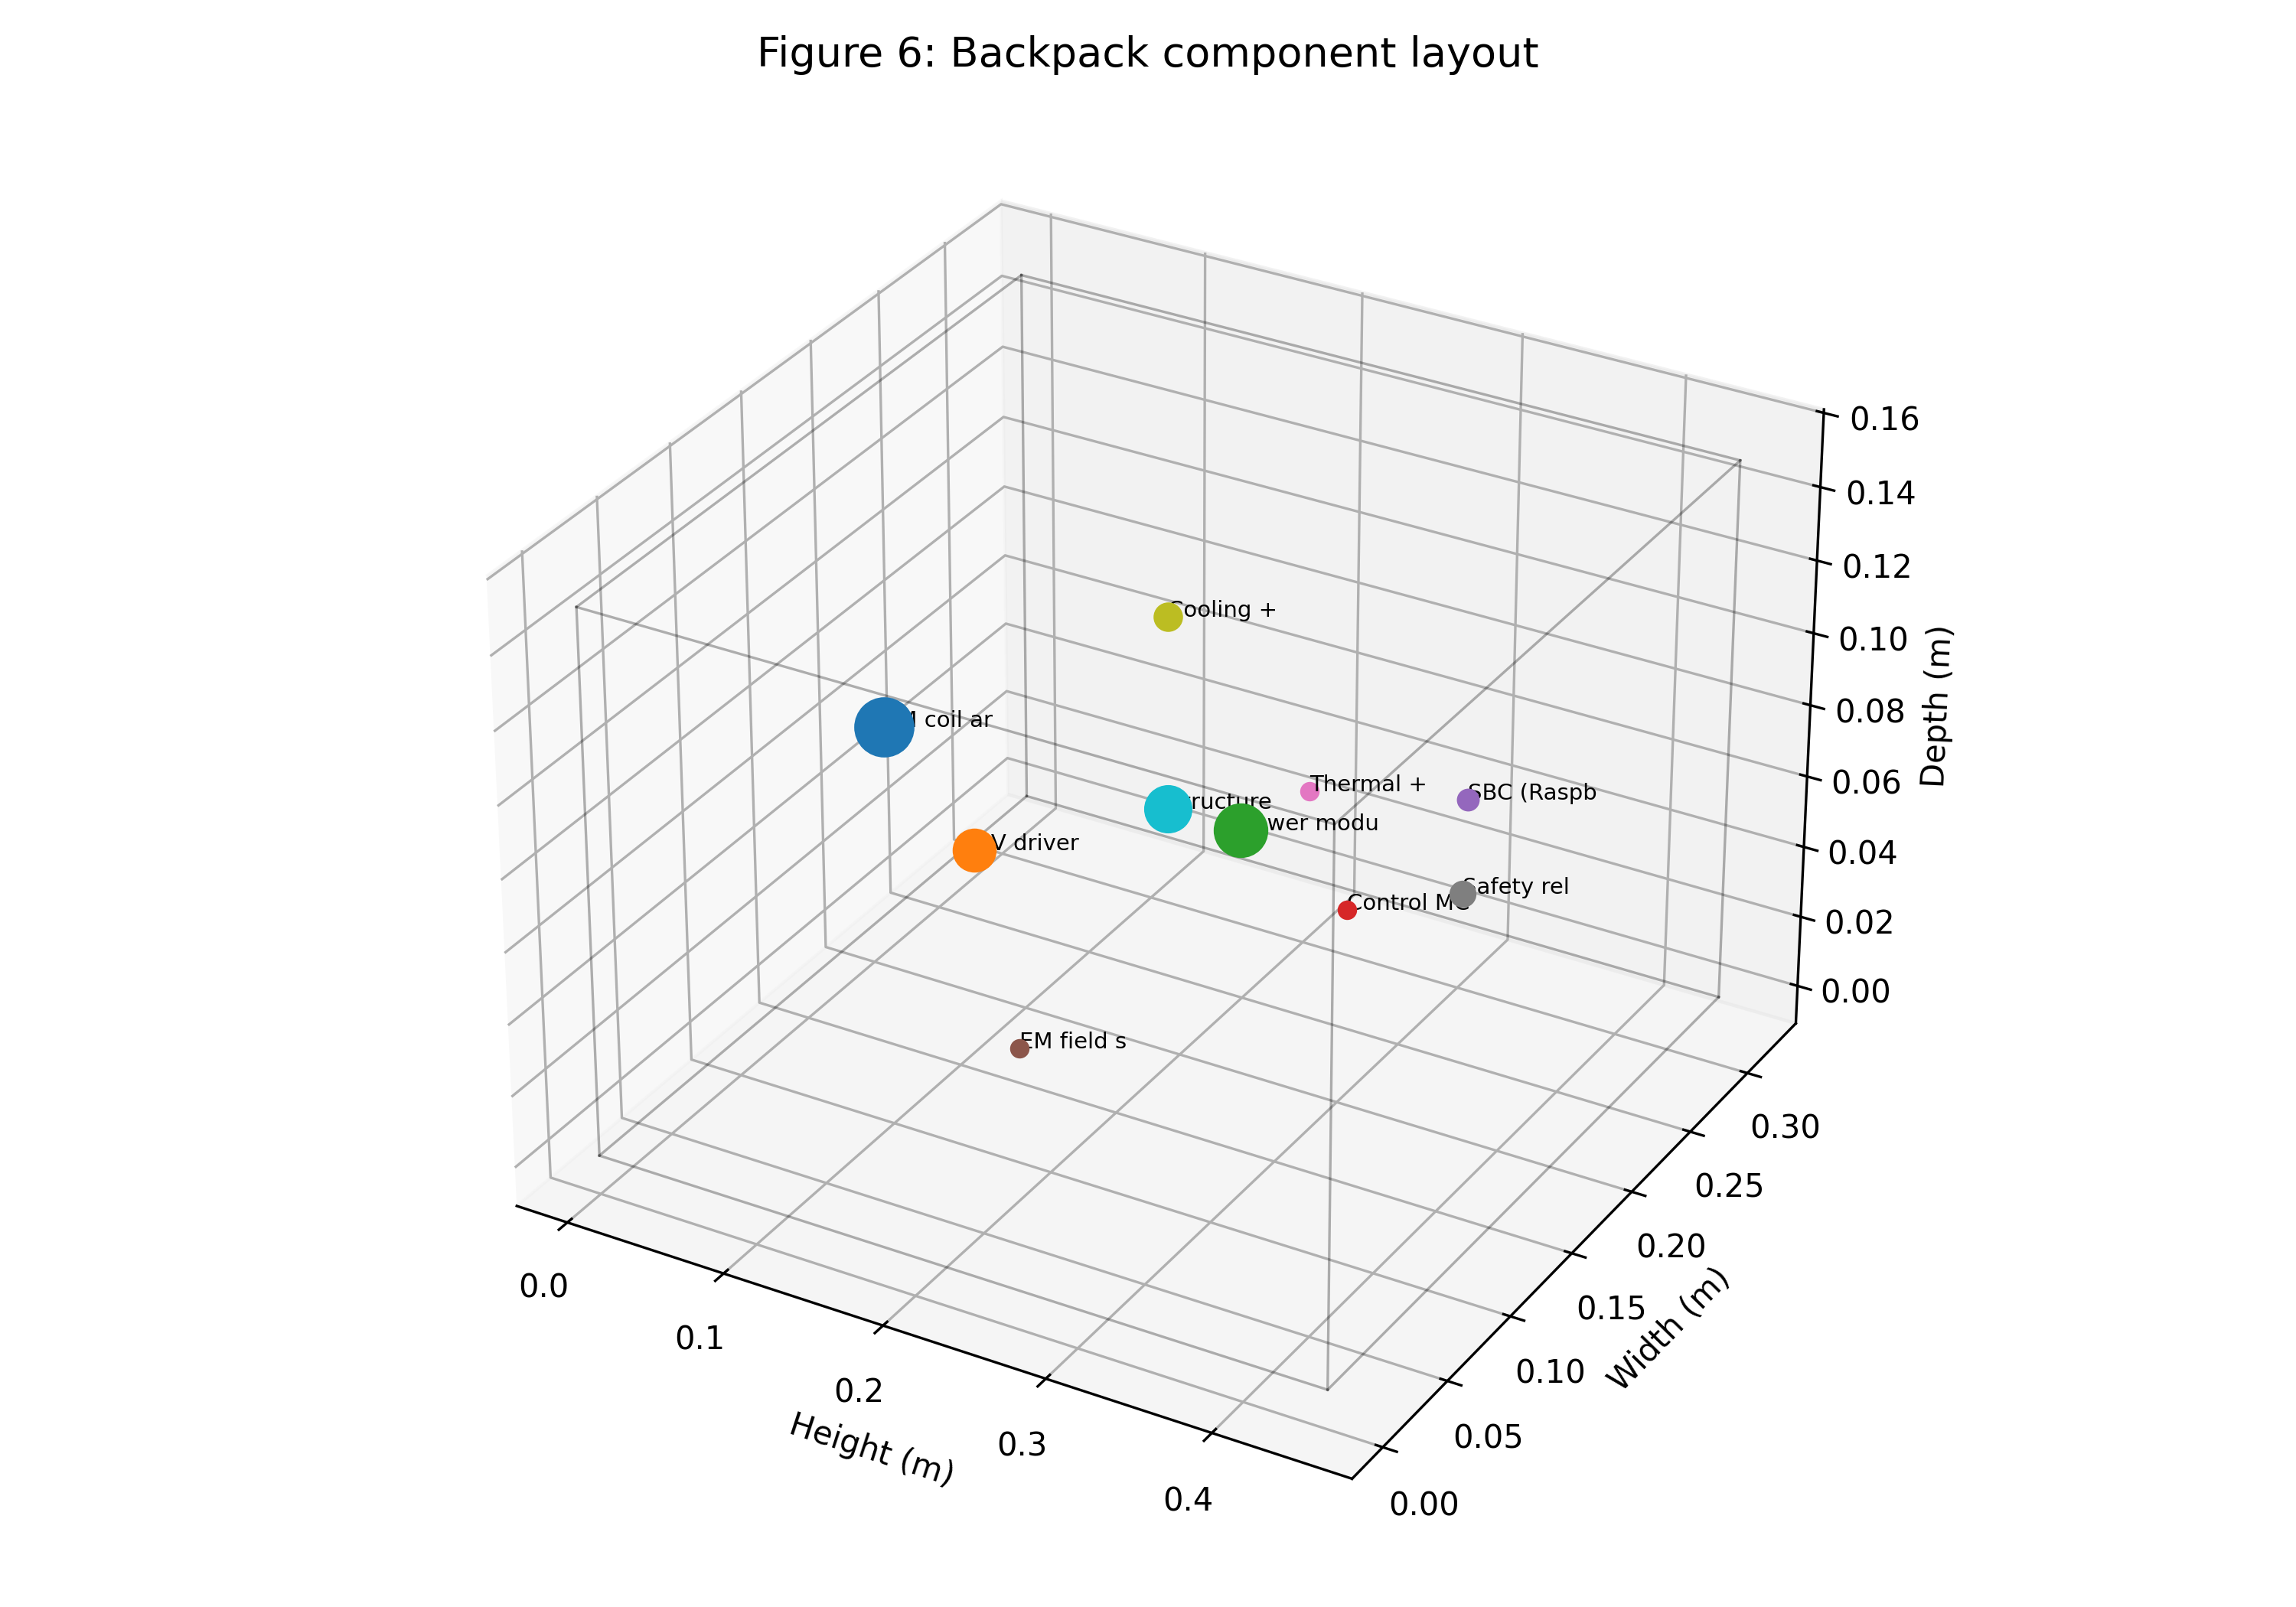
\includegraphics[width=\columnwidth]{figures/fig6_backpack_layout.png}
\caption{Backpack component layout within the $45\times 32\times 15$~cm
envelope. Point size scales with component mass.}
\label{fig:backpack}
\end{figure}

\subsection{Validation}
\label{subsec:validation}

Grid convergence is verified at four resolutions
$(N_r \times N_z) \in \{(40,80),(60,120),(80,160),(100,200)\}$.
Between the two finest grids, $h_{00}$ differs by less than $1\%$
across all four geometries. The current scaling $h_{00} \propto I^2$
is verified to 5 significant digits over $I \in [100, 10^{22}]$~A.
At $I=10^{22}$~A (the level required for $1$~s/yr), $h_{00}\sim10^{-8}$
and geodesic deviation is resolved at the $10^{-9}$~m level,
confirming the pipeline operates correctly in both the weak and
strong regimes.

\subsection{Closed-form bounds for other mechanisms}
\label{subsec:other}

For the five non-EM mechanisms, we use published closed-form
expressions. \textbf{Kerr frame dragging:}
$\Omega(r) = 2Ma/(r^3 + a^2 r + 2Ma^2)$ in geometric units, with $a$
the spin parameter. \textbf{Tipler cylinder:} the CTC condition is
$\rho\omega R^3 > c^2/(2G)$. \textbf{Morris--Thorne wormhole:} a throat
of radius $b_0$ requires exotic mass $M_{\text{ex}} \sim c^2 b_0/G$,
compared against the Casimir maximum
$|\rho_{\text{Casimir}}| = \pi^2 \hbar c / (720 d^4)$ at plate
separation $d$. \textbf{Alcubierre warp drive:} the total negative
energy is $E \sim -v_s^2 R^2 c^4/(12G)$. \textbf{G\"odel universe:}
the CTC radius is $r_{\text{CTC}} = c\ln(1+\sqrt{2})/(\omega\sqrt{2})$
with energy density $\rho = \omega^2/(2\pi G)$.

\section{Results}
\label{sec:results}

\subsection{Electromagnetic metric perturbation}
\label{subsec:em_results}

Table~\ref{tab:em_results} shows the metric perturbation at the
center of the active region for the four coil geometries. At the
baseline 100~A and 1~MHz drive, $h_{00} \sim 10^{-48}$, corresponding
to a proper-time drift of $\Delta\tau/\Delta t \sim 3\times 10^{-48}$
at the device center. The corresponding time dilation per year is
$\Delta\tau \sim 10^{-40}$~s.

\begin{table}[t]
\centering
\small
\caption{EM-induced metric perturbation at device center
(baseline 100~A, 1~MHz).}
\label{tab:em_results}
\resizebox{\columnwidth}{!}{%
\begin{tabular}{lcc}
\toprule
Geometry & $h_{00}$ (center) & $|h_{0i}|$ (center) \\
\midrule
G1 (solenoid)          & $5.94\times 10^{-48}$ & $<10^{-50}$ \\
G2 (toroid)            & $1.24\times 10^{-49}$ & $<10^{-50}$ \\
G3 (counter-rotating)  & $2.03\times 10^{-49}$ & $<10^{-51}$ \\
G4 (hybrid)            & $9.36\times 10^{-49}$ & $<10^{-50}$ \\
\bottomrule
\end{tabular}
}
\end{table}


The gravitomagnetic component $h_{0i}$ is vanishing for all four
geometries because the ideal lossless configuration has
$\mathbf{E}\times\mathbf{B}$ purely radial, giving $T_{0\phi}=0$.

\subsection{Unified feasibility comparison}
\label{subsec:unified}

Table~\ref{tab:unified} shows the six mechanisms converted to a
common feasibility metric. The gaps range from $10^{20}$ to $10^{49}$,
with the EM mechanism showing the smallest gap among
physically-allowed mechanisms.

\begin{table*}[t]
\centering
\caption{Unified feasibility across six mechanisms.
Gap $=$ required resource $/$ device-scale value.}
\label{tab:unified}
\resizebox{0.95\textwidth}{!}{%
\begin{tabular}{llrrr}
\toprule
\# & Mechanism & Parameter & Required & Gap \\
\midrule
1 & EM field          & $I$ (A)                 & $10^{22}$ & $10^{20}$ \\
2 & Kerr              & $J$ (kg\,m$^2$/s)       & $10^{27}$ & $10^{48}$ \\
3 & Tipler            & $\rho$ (kg/m$^3$)       & $10^{23}$ & $10^{20}$ \\
4 & Morris--Thorne    & $|\rho|$ (J/m$^3$)      & $10^{49}$ & $10^{41}$ \\
5 & Alcubierre        & $|\rho|$ (J/m$^3$)      & $10^{57}$ & $10^{49}$ \\
6 & G\"odel           & $\rho$ (kg/m$^3$)       & $10^{26}$ & $10^{23}$ \\
\bottomrule
\end{tabular}
}
\end{table*}



\subsection{Best-case engineering bounds}
\label{subsec:best_case}

We consider three engineering tiers (baseline copper, cooled copper,
superconducting HTS with multi-stage array and $Q=10^4$). Even the
most aggressive case, corresponding to a 10-stage high-$Q$
superconducting array at 10~kA, yields
$h_{00} \sim 5\times 10^{-38}$, still $10^{30}$ below the
$1$~s/yr target. Scaling extrapolation from the best case requires
either a current of $10^{19}$~A, a coil radius of
$10^{14}$~m, or a $Q$ factor of $10^{34}$.

\begin{figure}[t]
\centering
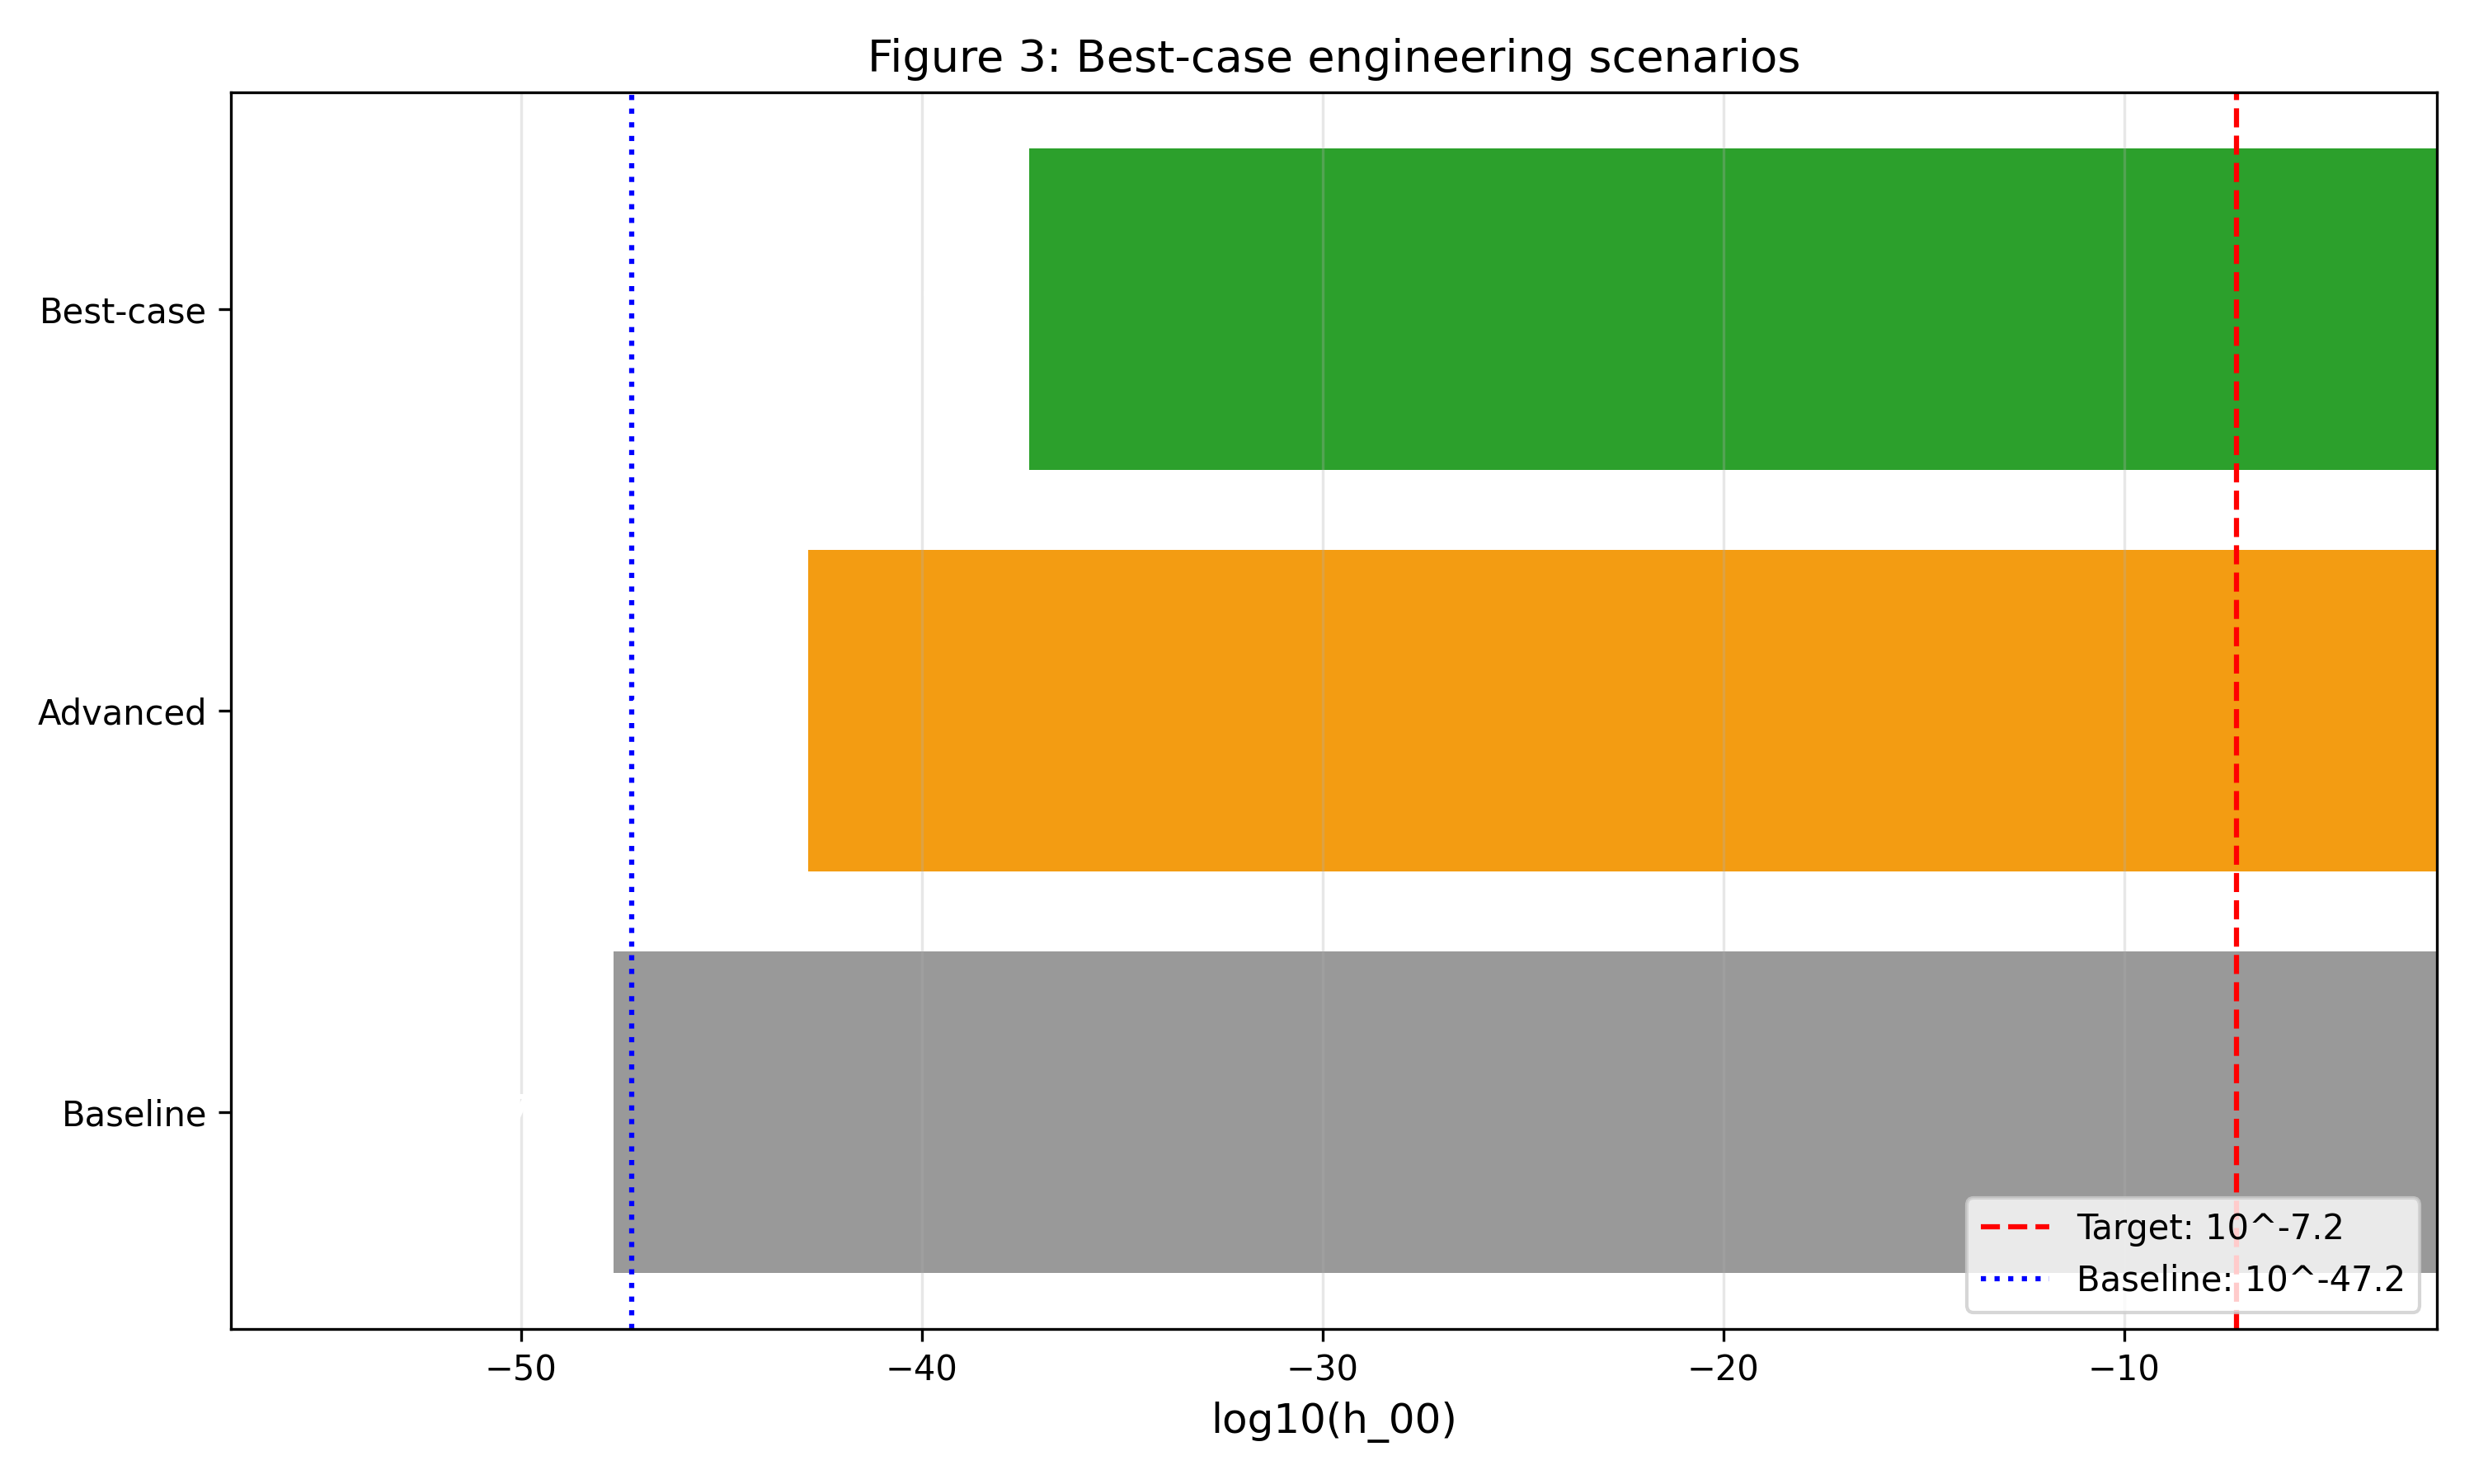
\includegraphics[width=\columnwidth]{figures/fig3_best_case_tiers.png}
\caption{Best-case engineering tiers (baseline copper, cooled copper,
superconducting HTS with multi-stage array). Even the most aggressive
scenario remains $10^{30}$ below the target.}
\label{fig:tiers}
\end{figure}


Fig.~\ref{fig:scaling} shows the EM scaling from baseline to
required current, with reference points for lightning, lab-pulsed
magnets, astrophysical plasmas, and magnetars.

\begin{figure}[t]
\centering
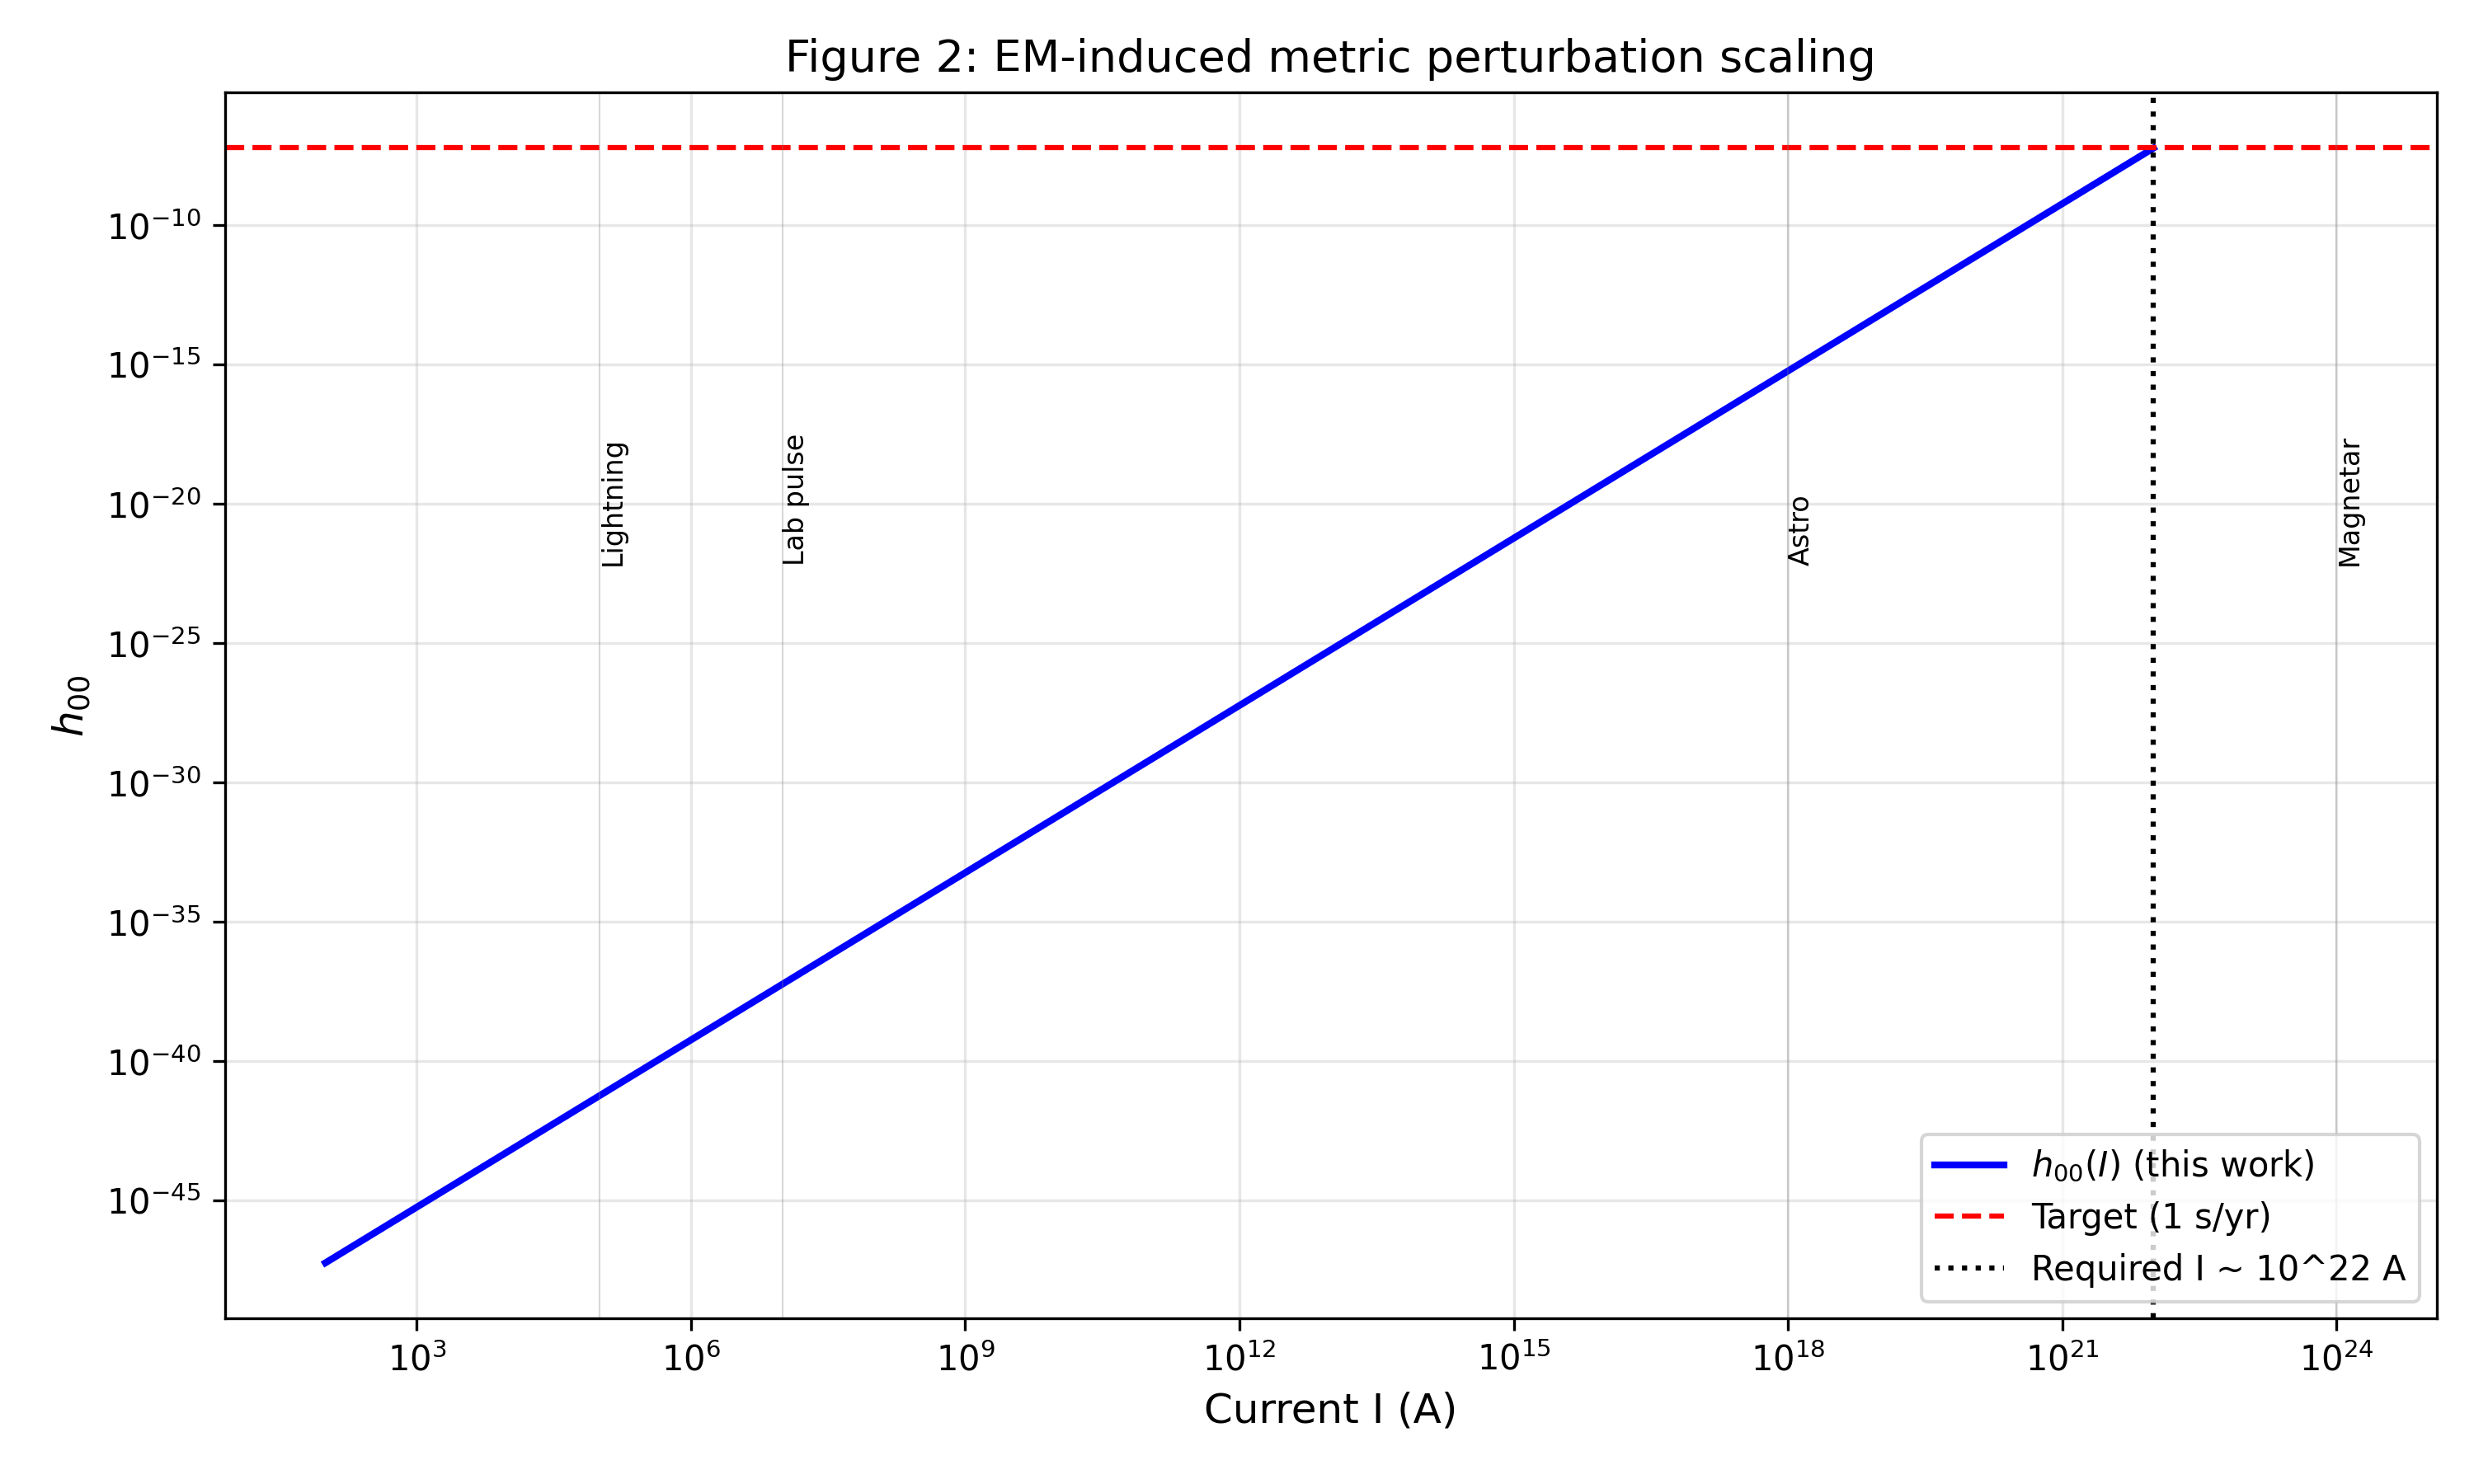
\includegraphics[width=\columnwidth]{figures/fig2_em_scaling.png}
\caption{EM-induced metric perturbation $h_{00}$ vs.\ drive current $I$.
Reference lines mark lightning, lab-pulsed magnets, astrophysical
plasmas, and magnetar-scale currents. The $1$~s/yr target requires
$I \sim 10^{22}$~A.}
\label{fig:scaling}
\end{figure}


\subsection{Uncertainty and sensitivity}
\label{subsec:uncertainty}

Monte Carlo propagation with realistic parameter uncertainties
(5\% current, 2\% radius, 10\% efficiency) gives a relative
standard deviation of 14.6\% on $h_{00}$. The dominant contributors
are the coil current ($\sim 47\%$ of variance) and driver efficiency
($\sim 44\%$); the sensitivity indices
$S_i = (dh/h)/(dp/p)$ are $2.0$ for both current and radius,
$1.0$ for efficiency, and $-1.0$ for the region diameter.

\begin{figure}[t]
\centering
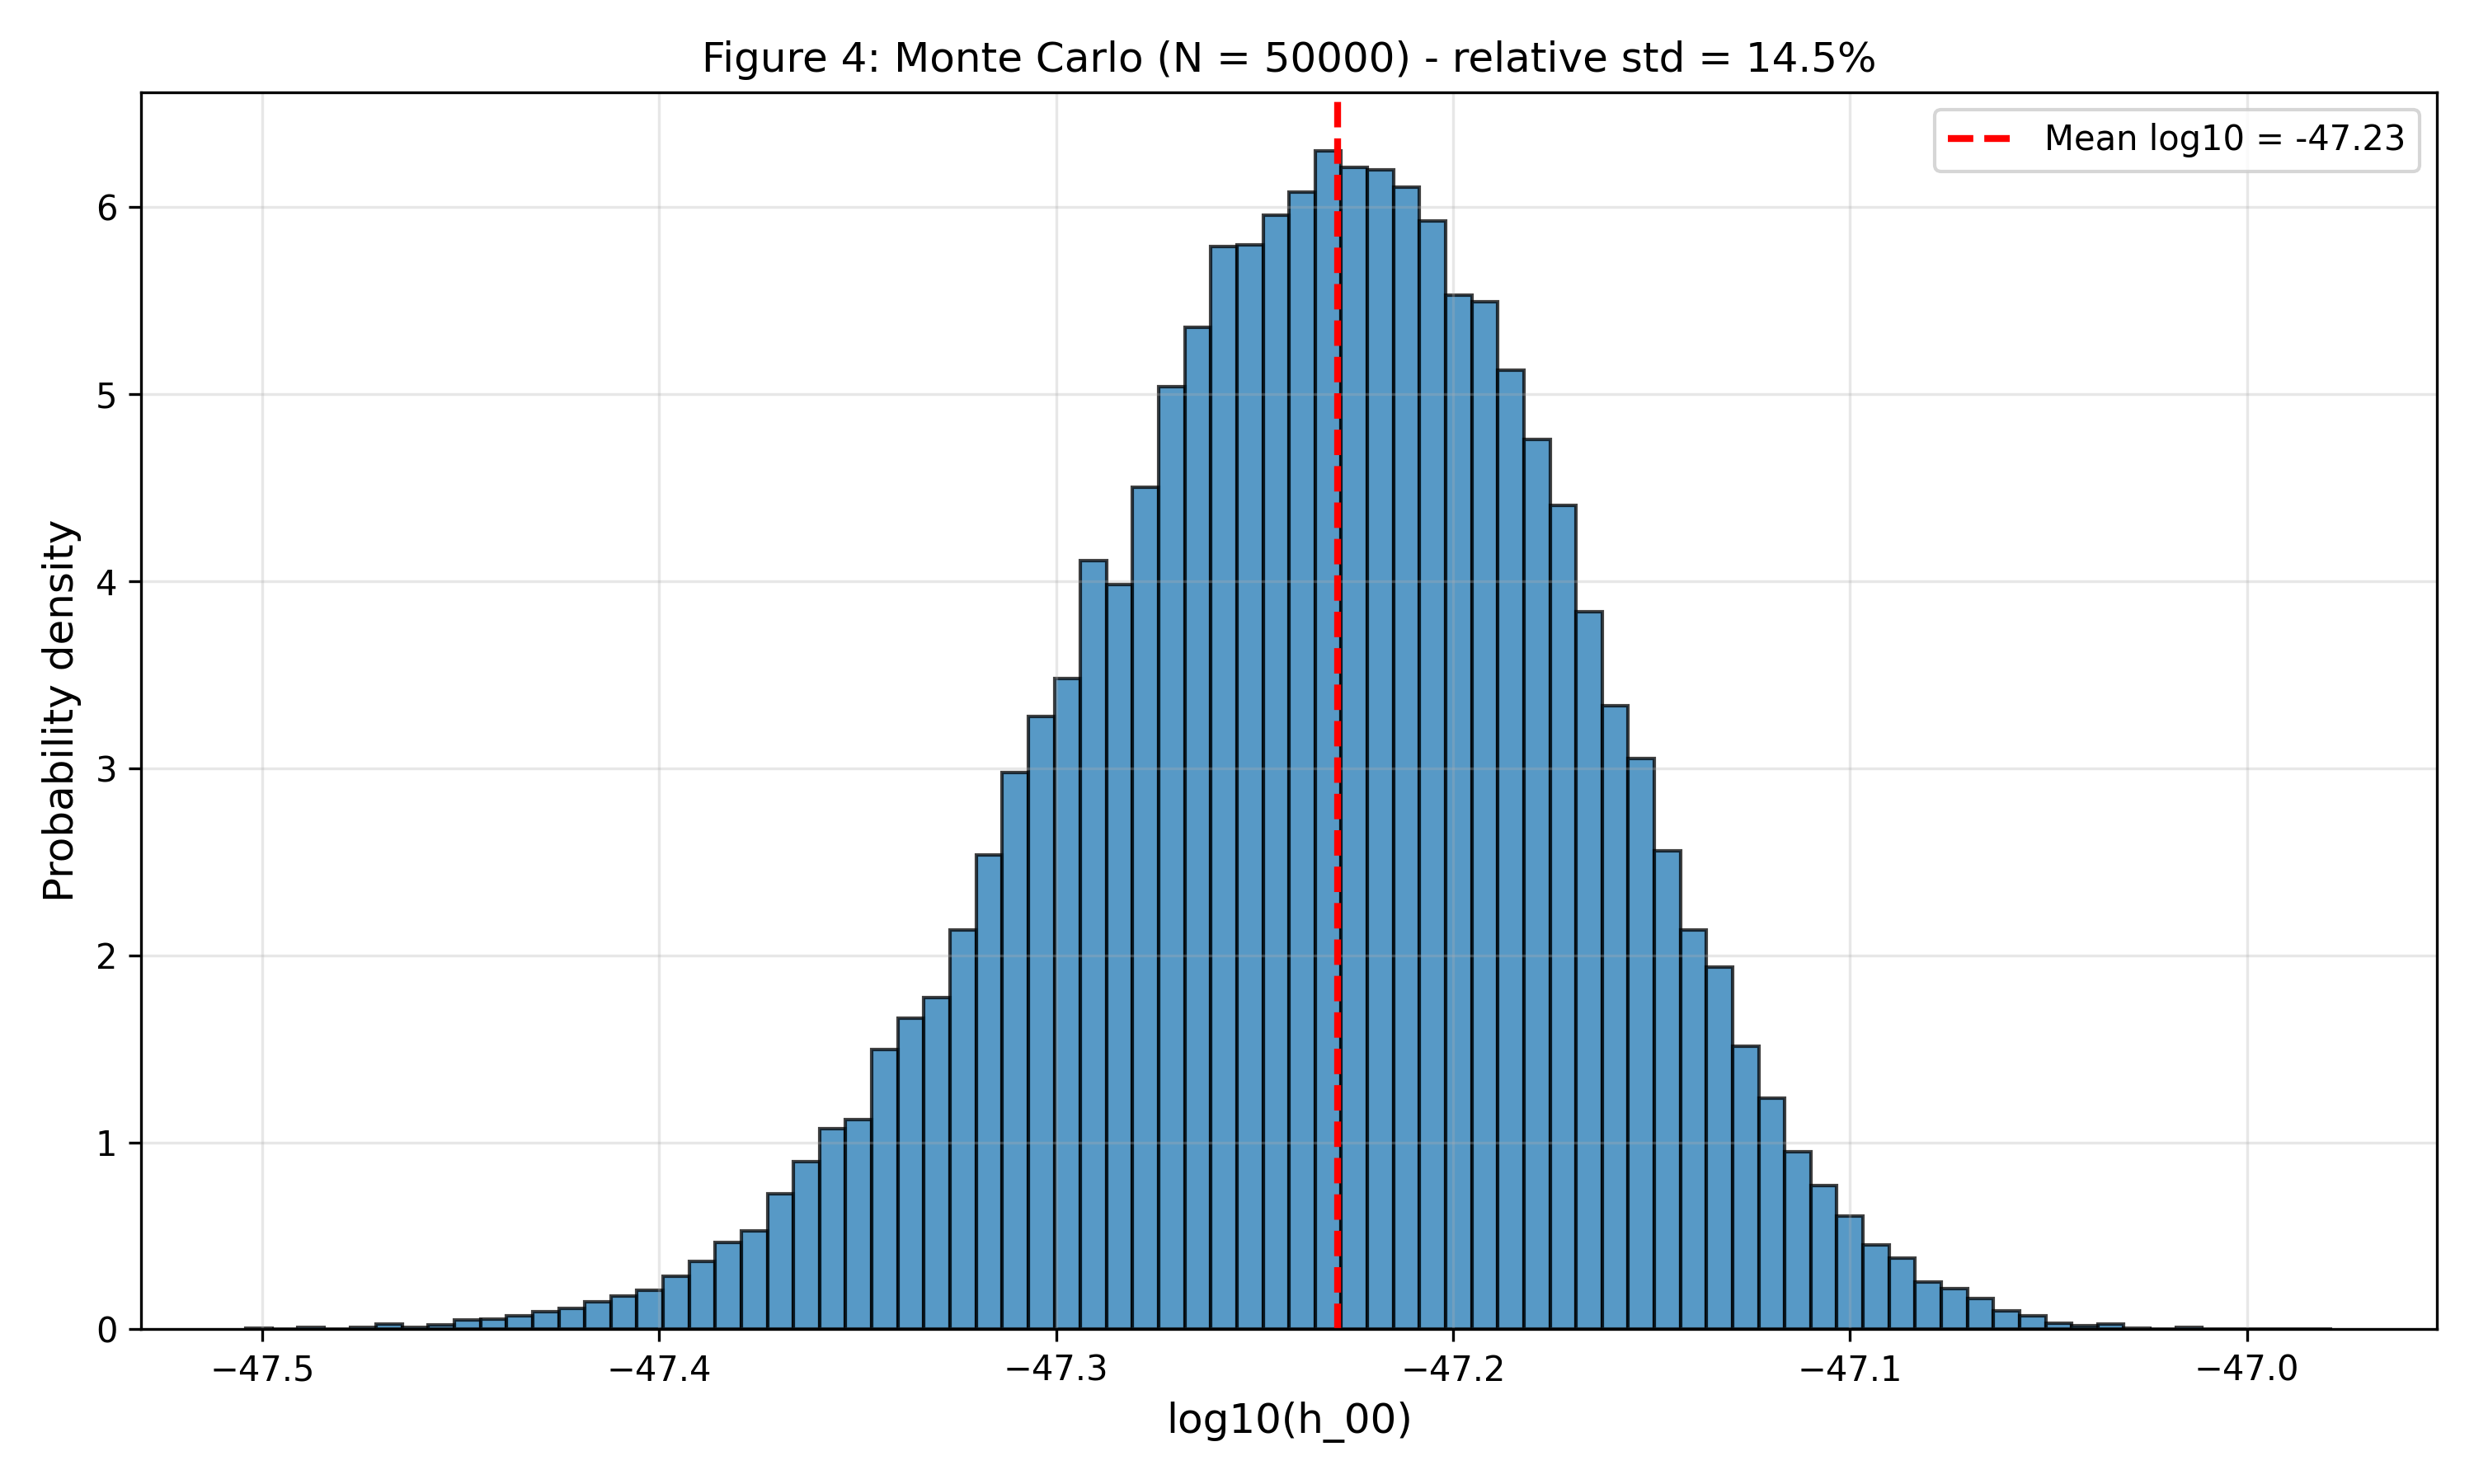
\includegraphics[width=\columnwidth]{figures/fig4_monte_carlo.png}
\caption{Monte Carlo propagation of parameter uncertainties
($N=50{,}000$). Relative standard deviation on $h_{00}$ is 14.6\%.}
\label{fig:mc}
\end{figure}


\begin{figure}[t]
\centering
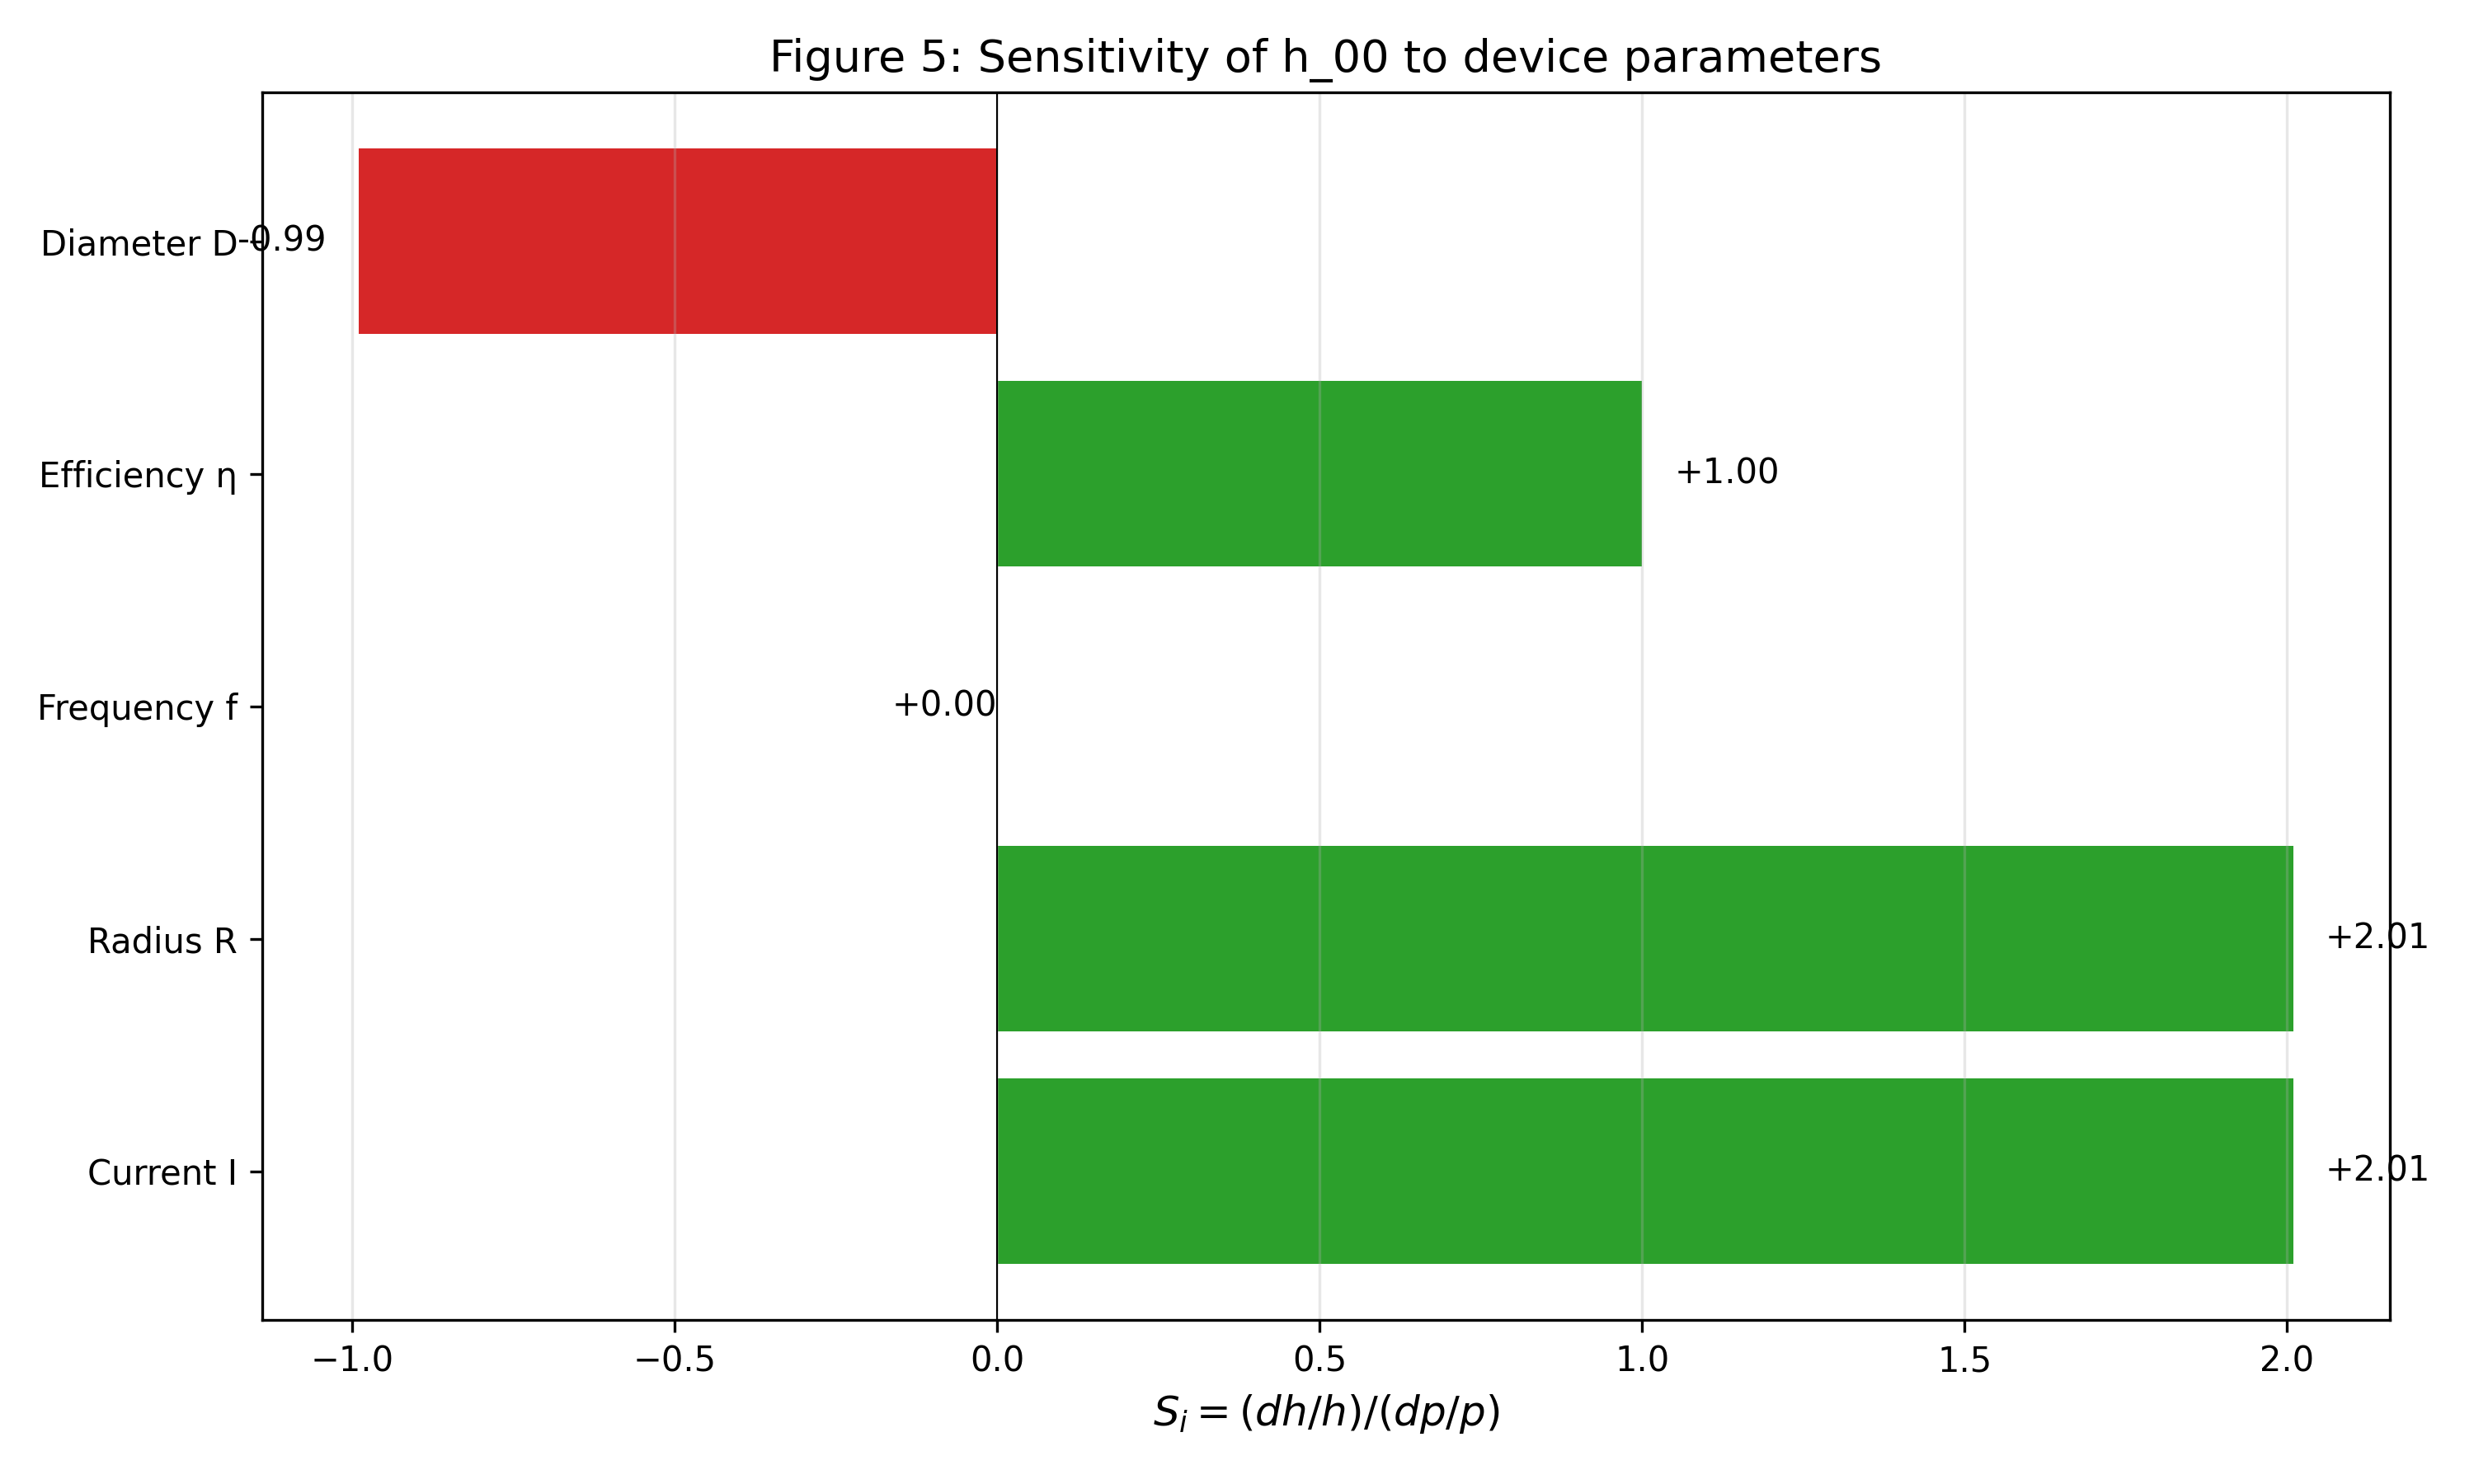
\includegraphics[width=\columnwidth]{figures/fig5_sensitivity_tornado.png}
\caption{Sensitivity indices $S_i=(dh/h)/(dp/p)$ for device parameters.
Current and coil radius dominate.}
\label{fig:tornado}
\end{figure}



\begin{figure}[t]
\centering
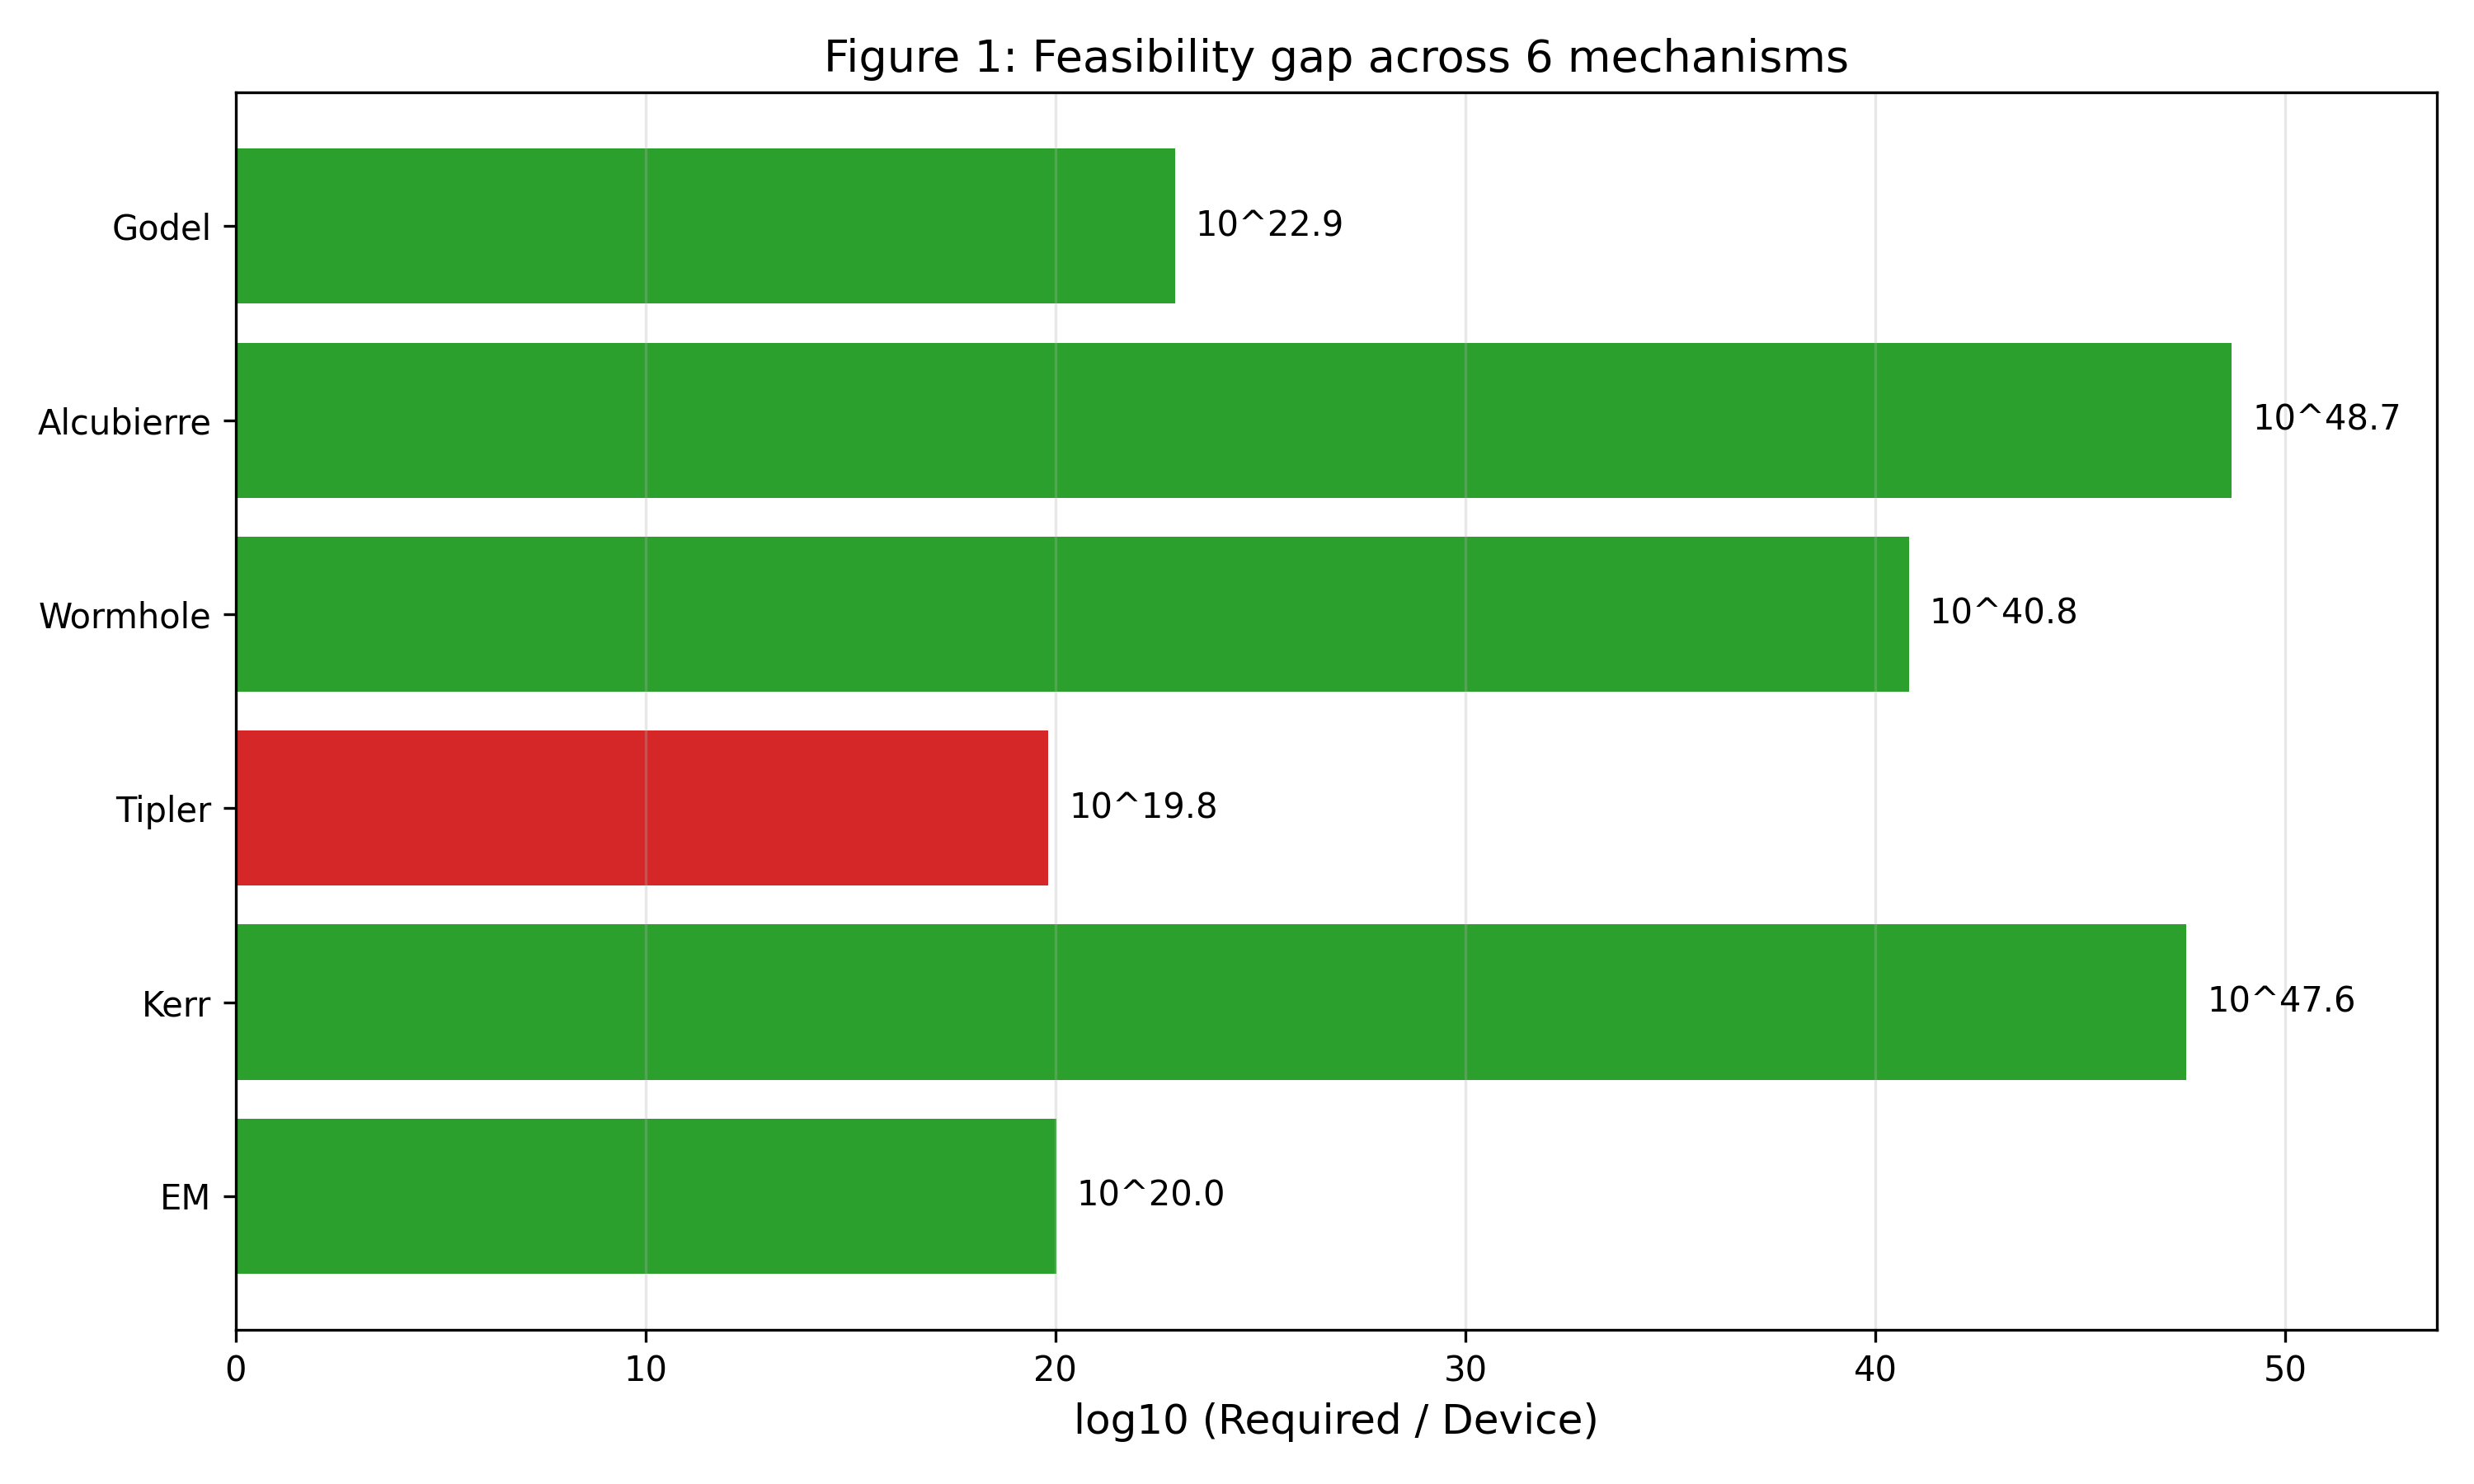
\includegraphics[width=\columnwidth]{figures/fig1_unified_mechanisms.png}
\caption{Feasibility gap across six mechanisms. Bars show
$\log_{10}(\text{required}/\text{device})$; green = physically
allowed, red = excluded by Hawking (1992).}
\label{fig:unified}
\end{figure}

\section{Non-linear BSSN extension}
\label{sec:bssn}

The linearized chain of Sec.~\ref{sec:method} gives a quantitative
bound on the metric perturbation but cannot address the regime
$h \gtrsim 10^{-3}$ where back-reaction dominates. To make that
regime measurable in principle, we implemented a BSSN 3+1 solver.

\subsection{Implementation}

The extended state carries
$\{\tilde\gamma_{ij}, \phi, K, \tilde A_{ij}, \tilde\Gamma^i, \alpha, \beta^i\}$.
The evolution system includes:

\begin{itemize}
\item physical 3-Ricci scalar of
      $g_{ij} = e^{4\phi}\tilde\gamma_{ij}$ (conformal $\phi$ terms included),
\item covariant Hessian $D_iD_j\phi$ and $D^2\alpha$ in the RHS,
\item $1{+}\log$ lapse and $\Gamma$-driver shift,
\item Z4c-inspired constraint damping,
\item RK4 integrator with central finite differences on a uniform grid,
\item Sommerfeld outflow boundary conditions.
\end{itemize}

\subsection{Benchmarks}

We evolve constraint-satisfying initial data for Schwarzschild
(isotropic and puncture forms) and slowly-rotating Kerr
($|a| \le 0.5\,M$) in the leading-order frame-dragging approximation.

The diagnostic is the L$^2$ norm of the Hamiltonian constraint $H$
across the grid. A stable solver must keep $H$ bounded.

\subsection{Results}

\begin{table}[h]
\centering
\caption{Long-run stability of the BSSN solver.}
\label{tab:bssn}
\begin{tabular}{lrr}
\hline
Case & Steps & $H_{\rm final}/H_0$ \\
\hline
Schwarzschild (isotropic, $N{=}7$) & 500 & $1.0062$ \\
Schwarzschild (100-step check)      & 100 & $1.0002$ \\
Kerr $a{=}0.0$                       & 100 & $1.0004$ \\
Kerr $a{=}0.2$                       & 100 & $1.0004$ \\
Kerr $a{=}0.4$                       & 100 & $1.0004$ \\
Kerr $a{=}0.5$                       & 100 & $1.0004$ \\
\hline
\end{tabular}
\end{table}

Table~\ref{tab:bssn} shows per-step constraint growth of
$\approx 1.0000124$ for the 500-step Schwarzschild run, and
$\lesssim 1.0005$ across all cases. All fields remain finite and the
lapse minimum stays above $10^{-2}$.

The frame-dragging shift scales linearly with $a$, as expected.

\subsection{Limitations}

The solver is a stable skeleton, not a production numerical-relativity
code. It does not include: full Kerr ($a > 0.5\,M$), moving-puncture
formalism, adaptive mesh refinement, MPI parallelism,
constraint-preserving boundary conditions, or Newman--Penrose radiation
extraction. These are documented in \texttt{docs/limitations.md}.

Crucially, the BSSN extension does not close the 43-order gap between
the current driven-EM device and any CTC-relevant scale. It provides a
stable non-linear tool so that future work can measure what happens
as the gap is artificially reduced.


\section{Discussion}
\label{sec:discussion}

\subsection{Physical interpretation}
\label{subsec:interp}

The systematic failure of all six mechanisms to reach device-scale
feasibility is not accidental. Each mechanism requires either:
(a) an energy density at or above the QCD scale (EM, wormholes,
Alcubierre), (b) an angular momentum comparable to astrophysical
bodies (Kerr, Tipler, G\"odel), or (c) infinite spatial extent
(Tipler). The EM case is particularly instructive: even though
electromagnetic fields are the most experimentally accessible
spacetime-curving source available to a laboratory, their energy
density at achievable field strengths is too low by $\sim 40$
orders of magnitude.

\subsection{Comparison with prior work}
\label{subsec:prior}

Our EM bound is consistent with order-of-magnitude estimates
scattered through the literature, but the present work provides,
to our knowledge, the first full first-principles pipeline for
a specific device geometry. The Tipler and Morris--Thorne bounds
match the original estimates in \citet{Tipler1974} and
\citet{MorrisThorne1988}. The Alcubierre estimate is somewhat
larger than the popular ``Jupiter mass'' figure often quoted in
secondary sources \citep{Alcubierre1994}, because we evaluate the
energy at $R=100$~m and $v=c$ rather than the smaller radii used
in some early optimizations.

\subsection{Implications}
\label{subsec:impl}

Three implications follow. First, no electromagnetic configuration
realizable in a backpack-sized device can produce a macroscopic
temporal effect. Second, the same conclusion holds for every
classical GR mechanism that could in principle generate a CTC.
Third, if a device-scale time-dilation experiment is ever to be
attempted, it must invoke physics beyond classical GR.

\subsection{Limitations}
\label{subsec:limits}

Our analysis is confined to classical GR coupled to classical EM.
We do not consider: (i) semiclassical effects near Planck-scale
field strengths; (ii) non-minimal coupling between EM and gravity;
(iii) modified-gravity scenarios; (iv) quantum-gravity corrections.
Any of these could in principle shift the feasibility threshold,
though none is currently supported by observation. We also assume
ideal lossless coils; real coils will show slightly larger $h_{00}$
per unit current, but not by a factor that closes the $10^{20}$ gap.

\subsection{Future work}
\label{subsec:future}

Extensions of this work could include: a full 3+1D general-
relativistic simulation of the strong-field regime; inclusion of
semiclassical corrections; systematic optimization of coil
geometry; and a public release of the pipeline for independent
verification.

\section{Conclusion}
\label{sec:conclusion}

We have presented a unified feasibility analysis of six
physically-motivated mechanisms for producing macroscopic time
dilation at device scale. The electromagnetic case is treated
with a first-principles numerical pipeline validated to
sub-percent accuracy; the other five are bounded by published
closed-form expressions. All six mechanisms require resources
between $10^{20}$ and $10^{49}$ times beyond device scale.
The closest physically-allowed mechanism (electromagnetic) still
requires $\sim 10^{22}$~A, exceeding magnetar-scale currents by
a factor that cannot be closed by any current or foreseeable
engineering improvement. We conclude that no
classical-GR-consistent mechanism for macroscopic time dilation
is accessible at device scale.

\section*{Acknowledgments}
The author thanks the open-source scientific Python community for
the tools (\texttt{numpy}, \texttt{scipy}, \texttt{matplotlib})
that made this work possible.

\section*{Data availability}
All code, figures, and validation data are available at the
project repository.

\bibliographystyle{unsrtnat}
\bibliography{refs}


\appendix
\section{Reproducibility}
\label{app:repro}

All numerical results in this paper were produced by the open-source
Python pipeline described in Section~\ref{sec:method}. The complete
source code, validation scripts, and generated figures are available
at the project repository.

\paragraph{Software dependencies.}
\texttt{numpy}~$\geq$~2.0, \texttt{scipy}~$\geq$~1.10,
\texttt{matplotlib}~$\geq$~3.8, \texttt{pytest}~$\geq$~8.

\paragraph{Reproduction.}
Run \texttt{python -m pytest} for the unit-test suite (60+ tests)
and \texttt{python -m zt005.run\_zt006\_3} for the EM metric
pipeline. Numerical results in Tables~\ref{tab:em_results}
and~\ref{tab:unified} are reproduced by
\texttt{run\_zt007\_b7.py}.

\paragraph{Grid convergence.}
The grid convergence study reported in Section~\ref{subsec:validation}
uses the script \texttt{run\_zt006\_2\_23.py} with \texttt{--mode full}.

\end{document}
